\documentclass{article}
\usepackage{tikz}
\usepackage{subfig}
\usepackage{graphicx}
\usepackage{xcolor}
\usepackage[margin=1.0in]{geometry}
\pagestyle{empty}

\definecolor{mygray}{rgb}{0.9, 0.9, 0.9} % Light gray

% TODO - stlpce s hranicami posunut dolava

\begin{document}

% % Add logo in the top-left corner
% \begin{tikzpicture}[remember picture, overlay]
%     \node at (0, 0) {\includegraphics[width=2cm]{stu-fei-vector-logo.png}};
% \end{tikzpicture}

% % Add name, ID, and date in a single line next to the logo
% \begin{flushright} % Use flushright to align text to the right
%     \textbf{Name: Your Name} \hspace{2em}
%     \textbf{ID: Your ID} \hspace{2em}
%     \textbf{Date: \today}
% \end{flushright}

% % Add text in the top-left corner
% \begin{tikzpicture}[remember picture, overlay]
%     \node[anchor=north, yshift=-2cm] at (current page.north) {
%         \textbf{Meno: Jozko Mrkvicka} \hspace{2em}
%         \textbf{ID: 120120} \hspace{2em}
%         \textbf{Dátum: \today}
%     };
% \end{tikzpicture}

% % Add logo in the top-left corner, optionally adjust position
% \begin{tikzpicture}[remember picture, overlay]
%     \node[anchor=north west, yshift=-0.5cm, xshift=2cm] at (current page.north west) {\includegraphics[width=2cm]{stu-fei-vector-logo.png}};
% \end{tikzpicture}
% % \vspace{1em} % Add some space below the header

\begin{tikzpicture}[remember picture, overlay]
    \node[anchor=north west, yshift=-0.2cm, xshift=2cm] at (current page.north west) {
        \parbox{20cm}{ % Adjust the width as necessary
            \includegraphics[width=2cm]{stu-fei-vector-logo.png} \hspace{2em} % Add the logo
            \textbf{Meno: Jozko Mrkvicka} \hspace{2em} % Add the name
            \textbf{ID: 120120} \hspace{2em} % Add the ID
            \textbf{Dátum: \today} % Add the date
            \\
            % \textbf{Miestnosť: CD300} % Add your new text
            % \textbf{Čas: 10:00}
        }
    };
\end{tikzpicture}


% Start of first column group
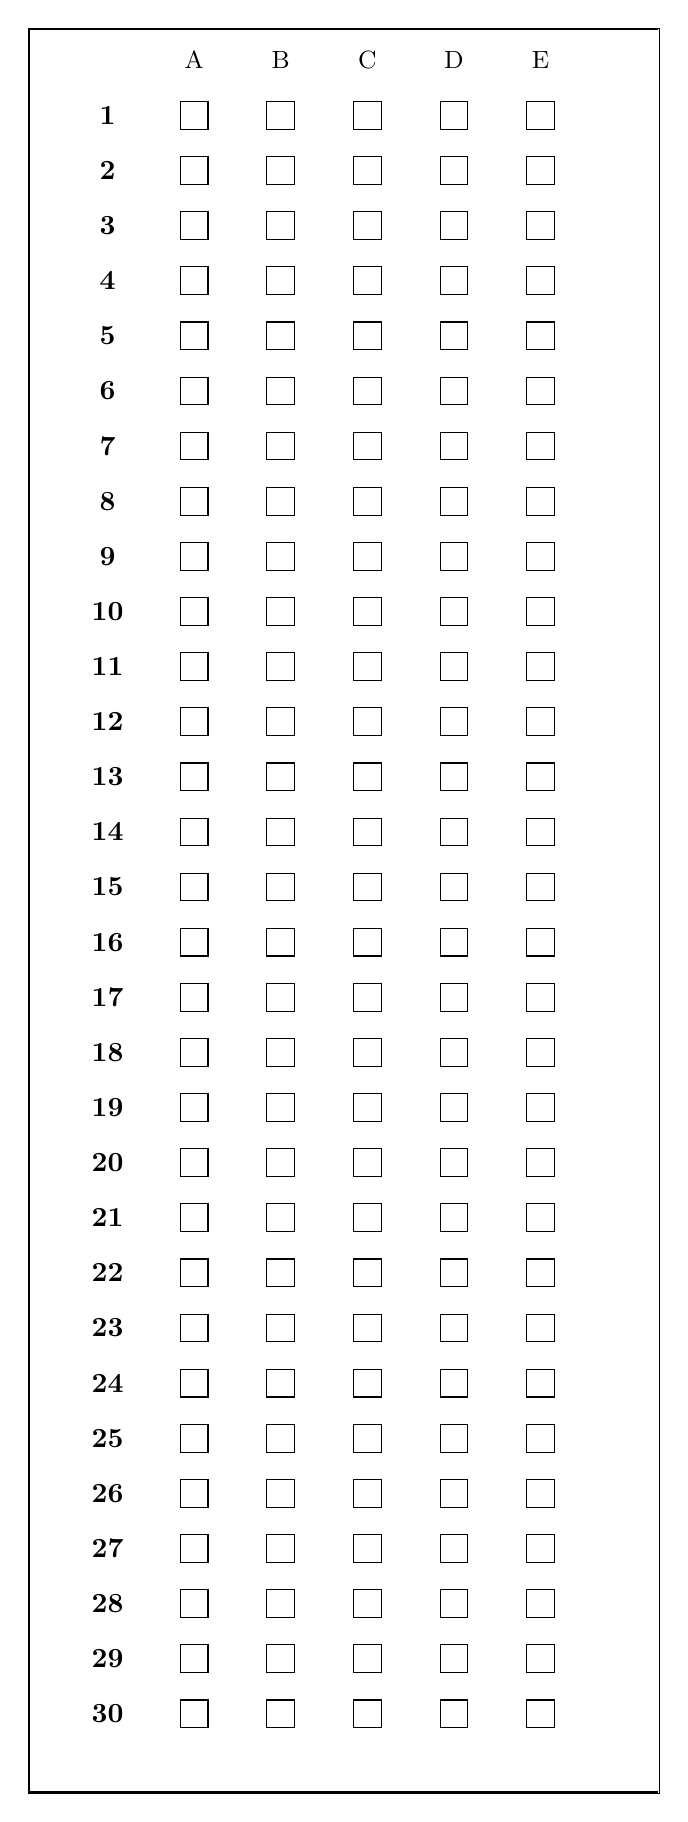
\begin{tikzpicture}[font=\small]

    % Draw column labels for the first large column
    \foreach \position/\letter in {1/A, 2/B, 3/C, 4/D, 5/E} {
        \node at ({\position * 1.1}, 0) {\letter}; % Position the letters above the squares
    }
    % Draw a black border around the first large column, extending it to include numbers
    
    \draw[thick, black] (-1, -22) rectangle (7, 0.4); % Extended the border to include line numbers

    % Draw the squares with gray crosses and line numbers in the first large column
    \foreach \line in {1,2,...,30} {
        \begin{scope}[yshift=-\line*0.7 cm]
            \node at (0,0) {\normalsize\textbf{\line}}; % Draw the line number (1 to 20)
            % Draw squares with gray crosses for each column
            \foreach \position in {1,2,3,4,5} { 
                \node[draw,rectangle,inner sep=5pt] at ({\position * 1.1},0) {}; % Empty squares
                % \node[mygray] at ({\position * 1.1},0) {\scalebox{1.1}{\textbf{$\times$}}};
                % \draw[red, thick] ({\position * 1.1}, 0) circle [radius=0.3cm]; % Add a red circle around each square
            }
        \end{scope}
          % Add a thin line every 5 records
        % \ifnum\line=5 \draw[thin, black] (-1,-\line*0.7 cm-0.35) -- (7,-\line*0.7 cm-0.35);\fi % After row 5
        % \ifnum\line=10 \draw[thin, black] (-1,-\line*0.7 cm-0.35) -- (7,-\line*0.7 cm-0.35);\fi % After row 10
        % \ifnum\line=15 \draw[thin, black] (-1,-\line*0.7 cm-0.35) -- (7,-\line*0.7 cm-0.35);\fi % After row 15
        % \ifnum\line=20 \draw[thin, black] (-1,-\line*0.7 cm-0.35) -- (7,-\line*0.7 cm-0.35);\fi % After row 20
        % \ifnum\line=25 \draw[thin, black] (-1,-\line*0.7 cm-0.35) -- (7,-\line*0.7 cm-0.35);\fi % After row 25
        % \ifnum\line=30 \draw[thin, black] (-1,-\line*0.7 cm-0.35) -- (7,-\line*0.7 cm-0.35);\fi % After row 30
    }
    
     \draw[white] (7, -22) -- (7, 0.4); % Separator line pre strednu dvojitu ciaru hrubu
\end{tikzpicture}\hfill
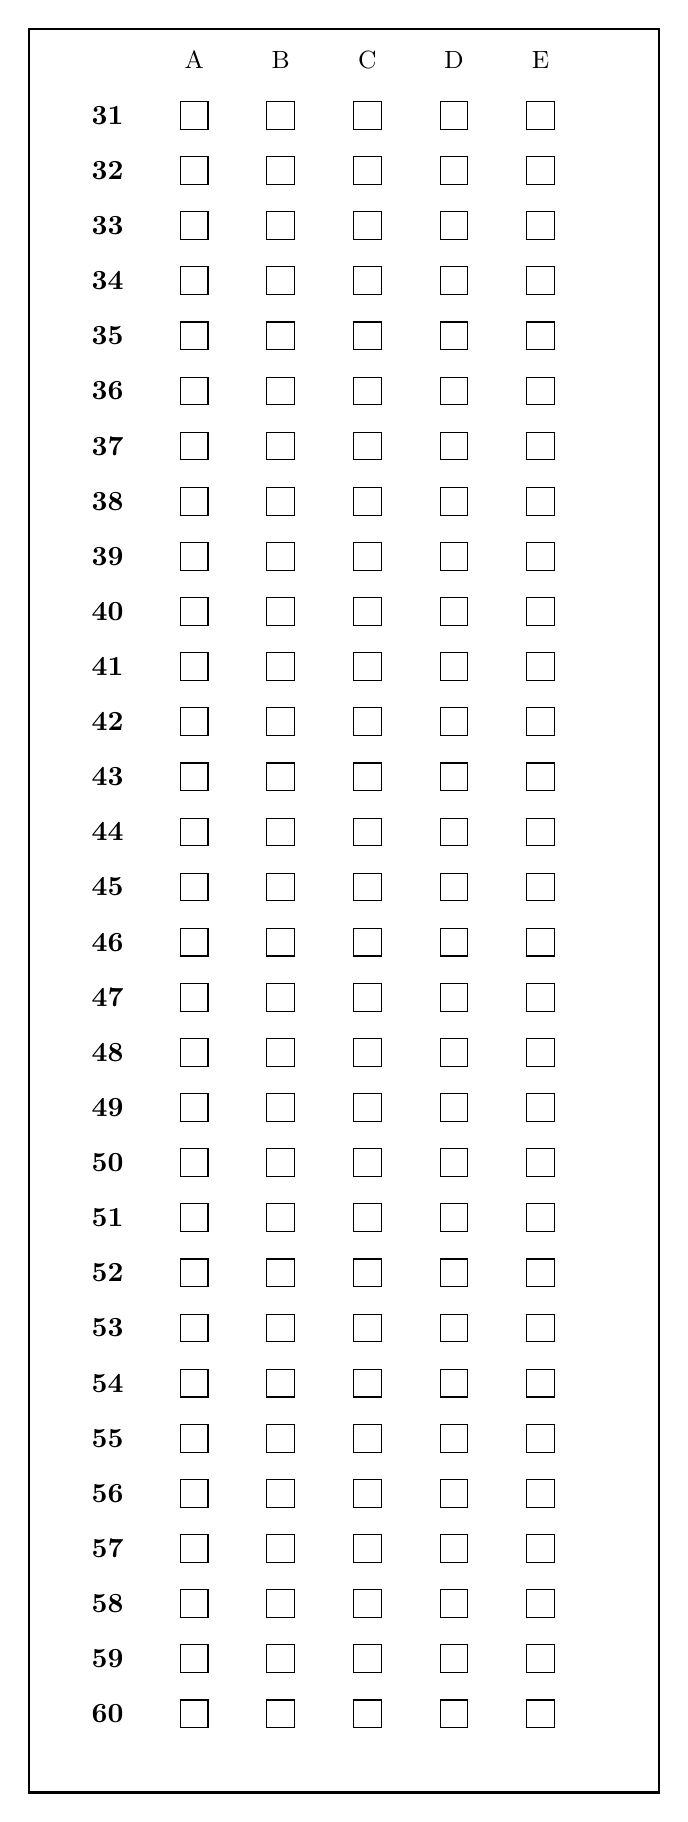
\begin{tikzpicture}[font=\small]

    % Draw column labels for the first large column
    \foreach \position/\letter in {1/A, 2/B, 3/C, 4/D, 5/E} {
        \node at ({\position * 1.1}, 0) {\letter}; % Position the letters above the squares
    }
    % Draw a black border around the first large column, extending it to include numbers
    
    \draw[thick, black] (-1, -22) rectangle (7, 0.4); % Extended the border to include line numbers

    % Draw the squares with gray crosses and line numbers in the first large column
    \foreach \line [count=\i from 1] in {31,32,...,60} { % Start numbering from 31 to 60
        \begin{scope}[yshift={-\i*0.7 cm}]
            \node at (0,0) {\normalsize\textbf{\line}};
            % Draw squares with gray crosses for each column
            \foreach \position in {1,2,3,4,5} { 
                \node[draw,rectangle,inner sep=5pt] at ({\position * 1.1},0) {}; % Empty squares
                % \node[mygray] at ({\position * 1.1},0) {\scalebox{1.1}{\textbf{$\times$}}};
                % \draw[red, thick] ({\position * 1.1}, 0) circle [radius=0.3cm]; % Add a red circle around each square
            }
        \end{scope}
    }
\end{tikzpicture}
\vfill

\end{document}
